\documentclass[../main.tex]{subfiles}

\begin{document}

\chapter[Vulnerabilities in Primal Decomposition-based dMPC]{Vulnerabilities in \\Primal Decomposition-based \\distributed \\Model Predictive Control}\label{sec:primal_decomposition}
\epigraph{\centering All the world\\ is birthday cake,\\ so take a piece, \\but not too much.}
{\textit{It's All Too Much}\\\textsc{George Harrison}}

In this chapter we describe in more details the optimization decomposition framework used in this work, giving insights of interpretation for each step.

Then we present the vulnerabilities of this framework illustrating some attacks and their consequences.

\minitoc

\newpage
\section{Primal decomposition-based \dmpc{}}\label{sec:decomposition_PD}

We start from the monolithic \mpc{} equivalent problem presented in~\eqref{eq:qp_standard_form}, which is reproduced here for the reader's convenience:
\begin{equation}
  \label{eq:qp_standard_form_reprise}
  \tag{\ref*{eq:qp_standard_form}}
  \begin{aligned}
    \begin{matrix}
      \minimize\limits_{\vec{U}[k]} &
      \frac{1}{2}\norm{\vec{U}[k]}^{2}_{H} + {\vec{f}[k]}^{T}\vec{U}[k] &\\
      \mathrm{subject~ to} &
\bar{\Gamma}\vec{U}[k]\preceq {\vec{U}}_{\text{max}}
    \end{matrix}
  \end{aligned}.
\end{equation}
As stated in \S\ref{sec:qp_mpc}, this problem is an input constrained \qp{} problem, which is convex.

To decompose the problem with the optimization decomposition frameworks shown in~\S\ref{sec:decomp-fram} we assume the objective function of problem~\eqref{eq:qp_standard_form_reprise} to be decomposable into $M$ equally sized parts, which correspond (corresponding sub-systems and sub-problems~\S\ref{sec:distributing_computation_units}) to sub divisions of the initial system~\eqref{eq:large_scale_system_model}.
The subsystems are ruled by dynamics $(A_{i},B_{i},C_{i})$, and have states $\vec{x}_{i}[k]$, references $\vec{w}_{i}[k]$ and inputs $\vec{u}_{i}[k]$.

Each sub-problem is given an index in set $\set{M}=\{1\mathbin{:}M\}$ and we rewrite~\eqref{eq:qp_standard_form_reprise} as
\begin{equation}
  \label{eq:qp_standard_form_decomposable}
  \begin{aligned}
    \begin{matrix}
      \minimize\limits_{\vec{U}_{1}[k],\dots, \vec{U}_{M}[k]} &
      \sum\limits_{i\in\set{M}}\left[\frac{1}{2}\norm{\vec{U}_{i}[k]}^{2}_{H_{i}} + {\vec{f}_{i}[k]}^{T}\vec{U}_{i}[k]\right]&\\
      \mathrm{subject~ to} & \sum\limits_{i\in\set{M}}\left[\bar{\Gamma}_{i}\vec{U}_{i}[k]\right] \preceq {\vec{U}}_{\text{max}}
    \end{matrix}
  \end{aligned},
\end{equation}
with local versions $\vec{U}_{i}[k]=\left[\vec{u}_{i}[0|k]; \dots; \vec{u}_{i}[\predhorz-1|k]\right]$, $\bar{\Gamma}_{i}$, $H_{i}$ and $\vec{f}_{i}[k]$ of variables presented in~\S\ref{sec:decomp-fram}.

\begin{remark}
  To pass from the global version of the variables in~\eqref{eq:qp_standard_form_reprise} to the local version in~\ref{eq:qp_standard_form_decomposable}, we apply a permutation transformation $Z^{T}Z=I$ to $\vec{U}[k]$ to reorder its components, such
  \begin{equation}
    \bar{\vec{U}}[k]=Z\vec{U}[k]=\left[\vec{U}_{1}[k]; \dots; \vec{U}_{M}[k]\right].
  \end{equation}
  Then we reorder other variables' elements consistently using the transformation.
  \begin{align}
    \label{eq:1}
    \bar{\bar{\Gamma}}&=\bar{\Gamma}Z^{T}=\left[\bar{\Gamma}_{1}, \dots, \bar{\Gamma}_{M}\right]\\
    \bar{\vec{f}}[k]&=Z\vec{f}[k]=\left[\vec{f}_{1}[k]; \dots; \vec{f}_{M}[k]\right]\\
    \bar{H}&=ZHZ^{T}=\blkdiag\limits_{i\in\set{M}} H_{i}
  \end{align}
\end{remark}

Using the methodology in~\S\ref{sec:generalizing_decomposition} for coupling constraints, the primal decomposition divides the problem~\eqref{eq:qp_standard_form_decomposable} into a main problem~\eqref{eq:DOP_main} and local problems~\eqref{eq:DOP_local} based on the original primal problem~\eqref{eq:qp_standard_form_decomposable} and using interface variables $\thetaik,\forall i\in\set{M}$:
\begin{subequations}
  \begin{equation}
        \eqoptobji(\thetaik)[k]=
        \begin{matrix}
          \minimize\limits_{\vec{U}_{i}[k]}&\frac{1}{2}\norm{\vec{U}_{i}[k]}^{2}_{H_{i}} + {\vec{f}_{i}[k]}^{T}\vec{U}_{i}[k]\\
          \mathrm{subject~ to} & \bar{\Gamma}_{i}\vec{U}_{i}[k] \preceq \thetaik:\lambdaik
      \end{matrix}
    \label{eq:DOP_local}
  \end{equation}

  \begin{equation}
    \begin{aligned}
      \eqoptobj[k]=
      \begin{matrix}
        \minimize\limits_{\mpcvec{\theta}[i][k], \dots, \mpcvec{\theta}[M][k]} &\sum\limits_{i\in\set{M}} J^{\star}_i(\thetaik)\\
        \mathrm{subject~ to} &
          \begin{aligned}
            \quad \sum_{i\in\set{M}}\thetaik\preceq\vec{U}_{\max}\\
          \end{aligned}
      \end{matrix}
    \end{aligned},
    \label{eq:DOP_main}
  \end{equation}
\end{subequations}
where $\lambdaik,\forall i\in\set{M}$ are the dual variables of the problems, i.e. the lagrange multipliers associated with the constraints~\cite{BoydVandenberghe2004}.

Problem~\eqref{eq:DOP_main} is solved by updating the $\theta_{i}$ until convergence. The method chosen is the projected sub-gradient, which update is given by
\begin{equation}
  \label{eq:projectedSubgradient}
\vec{\theta}[k]\pplusone=\Proj^{\set{S}}(\vec{\theta}[k]\p-\rho\p\vec{g}[k]\p),
\end{equation}
where $p$ is a given step in the iterative process, $\vec{\theta}[k]=[\vec{\theta}_{1}[k];\dots;\vec{\theta}_{M}[k]]$,
$\rho^{(p)}$ is a given step length,
${\set{S} = \setbuild{\vec{\theta}[k]}{I_{c}^{M}\vec{\theta}[k]\preceq \vec{U}_{\max}}}$,
${c=\card{\lambdaik}=\card{\thetaik}=\card{\vec{U}_{\max}}=n_{c}\predhorz}$,
${I_{c}^{M}=\kron{\1_{M}\T}{I_{c}}}$,
and
$\vec{g}\p[k]$ is a sub-gradient of the objective function of problem in~\eqref{eq:DOP_main} in step $p$.
The choice of the step length is given such
\[\lim_{p\to\infty}\rho^{(p)}\to0\]
and
\[\sum_{p=1}^{\infty}\rho^{(p)}\to\infty.\]
An usual law is
\begin{equation}
  \label{eq:rho_update}
  \rho^{(p)}=\frac{1}{a+bp},
\end{equation}
with $a$ and $b$ arbitrarily chosen~\cite{ConejoEtAl2006}.

From~\cite{BoydVandenberghe2004} and~\cite{BoydEtAl2015}, we can derive that the opposite of the dual variables $\lambdaik$ of the local problems are sub-gradients of the local problems and since the objective function of the main problem is a sum of the local objectives, then the $\vec{\lambda}_{i}$ can form a sub-gradient of the main problem.
If we stack the $\vec{\lambda}_{i}[k]$ in $\vec{\lambda}[k]=[\vec{\lambda}_{1}[k];\dots;\vec{\lambda}_{M}[k]]$, it can be used in~\eqref{eq:projectedSubgradient}, yielding
\begin{equation}
  \label{eq:projectedSubgradient_lambda}
  \vec{\theta}[k]\pplusone=\Proj^{\set{S}}(\vec{\theta}[k]\p+\rho\p\vec{\lambda}[k]\p).
\end{equation}

Using~\eqref{eq:DOP_local} and~\eqref{eq:projectedSubgradient_lambda}, we can alter Algorithm~\ref{alg:decomposition_coordination} to correspond to a decomposition of the original \mpc{} problem~\eqref{eq:qp_standard_form_decomposable} using the primal decomposition:
\begin{algorithm2e}[h]
  \DontPrintSemicolon%
  \KwIn{Maximum number of iteration $p_{\max}$, Bound $\epsilon$,Constants $a$ and $b$}
  \KwOut{Optimal allocations $\vec{\theta}[k]$}
  $p\gets 0$\;
  Initialize ${\thetaik}^{(p)},$ $\forall i\in\set{M}$, such that ${\vec{\theta}[k]}^{(p)}\in\set{S}$\;
  \Repeat{$\left[\norm{{\vec{\theta}[k]}^{(p)}-{\vec{\theta}[k]}^{(p-1)}}\leq\epsilon\right]\lor \left[p\geq p_{\max}\right]$}{
    Solve local sub-problems~\eqref{eq:DOP_local} and calculate ${\vec{\lambda}_{i}[k]}^{(p)}$ (potentially in parallel)\;
    Update $\vec{\theta}[k]$: $\vec{\theta}[k]\pplusone\gets\Proj^{\set{S}}(\vec{\theta}[k]\p+\rho\p\vec{\lambda}[k]\p)$ \;
    $p\gets p+1$\;
  }
  \caption{Decomposition of \mpc{} problem using primal decomposition.}\label{alg:primal_decomposition}
\end{algorithm2e}

Since each problem~\eqref{eq:DOP_local} can potentially be solved in parallel, a different computation unit is allocated to solve each problem.
For the update~\eqref{eq:projectedSubgradient_lambda} the agents need to have the $\lambdaik$ of all other agents to update the $\thetaik$.
We could create an anarchic solution analog to the one in~\cite{VelardeEtAl2018} where the $\lambdaik$ information circulate among agents and each agent update its own $\thetaik$.
However, we decide for a more private structure.
We choose to use an \textbf{hierarchic} solution, allocating another agent to aggregate the $\lambdaik$ and coordinate the updates of the $\thetaik$, we called this agent the \emph{coordinator}.
This way, each agent has only access to its own $\lambdaik$ and $\thetaik$.

We can illustrate the communication structure using Fig.~\ref{fig:dmpc_communication}, which is the same in our introductory example.
We summarize the complete primal decomposition-based \dmpc{} algorithm in Algorithm~\ref{alg:primal_decomposition_based_dmpc}.

\begin{algorithm2e}[h]
  \DontPrintSemicolon%
  \coordinit{
    Initialize $k$, $p$, $a$, $b$, $p_{\max}$ and $\epsilon$\;
  }
  \While{$k\geq 0$}{
    Initialize ${\thetaik}^{(p)},$ $\forall i\in\set{M}$, such that ${\vec{\theta}[k]}^{(p)}\in\set{S}$\;
    Coordinator sends $\thetaik^{(p)}$ for all agents\;
    \exchange{
      \Repeat{$\left[\norm{{\vec{\theta}[k]}^{(p)}-{\vec{\theta}[k]}^{(p-1)}}\leq\epsilon\right]\lor \left[p\geq p_{\max}\right]$}{
        Agents solve local sub-problems~\eqref{eq:DOP_local} and send ${\vec{\lambda}_{i}[k]}^{(p)}$ to coordinator\;
        Coordinator updates $\vec{\theta}[k]$ using~\eqref{eq:projectedSubgradient_lambda} and sends to local agents\;
        $p\gets p+1$\;
      }
    }
    Agents apply on respective sub-systems the last calculated $\vec{u}_{i}^{\star}[0|k]$\;
    $k\gets k+1$\;
  }
  \caption{Primal decomposition-based \dmpc{}.}\label{alg:primal_decomposition_based_dmpc}
\end{algorithm2e}

\begin{figure}[H]
  \centering
  \begin{tikzpicture}[font=\small,thick,node distance=3*0.6180cm and 0.6180cm,every node/.style=rectangle,
    mpcSmall/.style={fill=mpc_agent, minimum height=0.6180*2cm, minimum width=2cm},
    coordinator/.style={fill=mpc_coordinator, minimum height=0.6180*3cm, minimum width=6cm},
    ]

    \node[draw, mpcSmall,] (block1) {\small Agent 1};
    \node[fill=none, draw=none, right=of block1,] (mult) {\bf $\dots$};
    \node[draw, mpcSmall, fill=mpc_agent, right=of mult,] (blockM) {\small Agent M};
    \node[draw, coordinator, below=of mult,] (coordinator) {Coordinator};

    \draw[-latex,line width=1pt] (block1.south)+(0.4,.0) -- ( coordinator.north -| {$(block1.south)+(0.4,.0)$}) node [right,midway] {$\lambda_{1}$};
    \draw[latex-,line width=1pt] (block1.south)+(-0.4,0) -- (  coordinator.north -| {$(block1.south)+(-0.4,0)$}) node [left,midway] {$\theta_{1}$};
    \draw[-latex,line width=1pt] (blockM.south)+(0.4,.0) -- ( coordinator.north -| {$(blockM.south)+(0.4,.0)$}) node [right,midway] {$\lambda_{M}$};
    \draw[latex-,line width=1pt] (blockM.south)+(-0.4,0) -- (  coordinator.north -| {$(blockM.south)+(-0.4,0)$}) node [left,midway] {$\theta_{M}$};
  \end{tikzpicture}
  \caption{Exchange between local controllers and coordinator in Primal decomposition-based \dmpc{}.}\label{fig:dmpc_communication}
\end{figure}

\begin{remark}
  The same decomposition can be used if the coupling constraints are equalities or if there are local constraints for the subsystems.
  We can change problems~\eqref{eq:DOP_local} and~\eqref{eq:projectedSubgradient_lambda} accordingly to respect such modifications, i.e.\ adding the local constraints to the local problems and changing the inequality constraints to equality ones, including in the set $\set{S}$.
  Examples of each are given in the next section and chapters.
\end{remark}

\section{Example and Interpretations}\label{sec:example-interpr}
As a simple numerical example to illustrate the functioning of the algorithm we take $M=3$ \mbox{$1$-dimensional} \siso{} ($n_{x}=1$,$n_{c}=1$) systems coupled by the inputs.
The systems have no physical meaning but due to their small scale it is easier to visualize.

The systems are described by the following \ltidt{} dynamics
\begin{equation}
  \label{eq:example_dynamics}
  x_{i}[k+1]=a_{i}x_{i}[k]+b_{i}u_{i}[k]
\end{equation}
where
$a_1=0.8$, $a_2=0.6$, $a_3=0.4$, $b_1=0.3$, $b_2=0.5$, and $b_3=0.6$,
The system is
constraint by an equality constraint
\begin{equation}
  \label{eq:example_equality}
  u_{1}+u_{2}+u_{3}=\vec{u}_{\max}
\end{equation}
with
$\vec{u}_{\max}=4$
.

We use a \dmpc{} with horizon ${\predhorz=2}$,
initial conditions
${x_{1}[0]=3}$, 
${x_{2}[0]=2}$, 
and 
${x_{3}[0]=1}$

and state references
${w_{1}[0]=\frac{107}{100}x_{1}[0]}$, 
${w_{2}[0]=\frac{11}{10}x_{2}[0]}$, 
and 
${w_{3}[0]=\frac{21}{20}x_{3}[0]}$

and gains
$Q_{i}=10I_{2}$ and
$R_{i}=   I_{2}$
that results in the problems
\begin{equation}
    \eqoptobji(\thetaik)[k]=
    \begin{matrix}
    \minimize\limits_{\vec{U}_{i}[k]}&\frac{1}{2}\norm{\vec{U}_{i}[k]}^{2}_{H_{i}} + {\vec{f}_{i}[k]}^{T}\vec{U}_{i}[k]\\
    \mathrm{subject~ to} & \bar{\Gamma}_{i}\vec{U}_{i}[k] = \thetaik:\lambdaik
  \end{matrix}
  \label{eq:example_local_problem}
\end{equation}
with
\begin{equation}
  \label{eq:1}
  \begin{array}{lll}
    H_1=\left(\begin{array}{cc} \frac{6077}{3125} & \frac{288}{625}\\ \frac{288}{625} & \frac{197}{125} \end{array}\right), & \vec{f}_1[k]=\left(\begin{array}{c} \frac{1968}{625}\\ \frac{192}{125} \end{array}\right)x_i[k]-\left(\begin{array}{cc} \frac{12}{5} & \frac{48}{25}\\ 0 & \frac{12}{5} \end{array}\right)\vec{W}_i[k], & \bar{\Gamma}_1=I_2,\\\\
H_2=\left(\begin{array}{cc} \frac{278}{125} & \frac{27}{50}\\ \frac{27}{50} & \frac{19}{10} \end{array}\right), & \vec{f}_2[k]=\left(\begin{array}{c} \frac{306}{125}\\ \frac{27}{25} \end{array}\right)x_i[k]-\left(\begin{array}{cc} 3 & \frac{9}{5}\\ 0 & 3 \end{array}\right)\vec{W}_i[k], & \bar{\Gamma}_2=I_2,\\\\
H_3=\left(\begin{array}{cc} \frac{5213}{3125} & \frac{144}{625}\\ \frac{144}{625} & \frac{197}{125} \end{array}\right), & \vec{f}_3[k]=\left(\begin{array}{c} \frac{696}{625}\\ \frac{48}{125} \end{array}\right)x_i[k]-\left(\begin{array}{cc} \frac{12}{5} & \frac{24}{25}\\ 0 & \frac{12}{5} \end{array}\right)\vec{W}_i[k], & \bar{\Gamma}_3=I_2.\\\\

  \end{array}
\end{equation}
The coordinator update function is the same as~\eqref{eq:projectedSubgradient_lambda} but with ${\set{S} = \setbuild{\vec{\theta}[k]}{I_{c}^{M}\vec{\theta}[k] = \vec{U}_{\max}}}$, where $c=2$.

From now on, we remove the $[k]$ indices for convenience, since all calculation is for the same step $k$ unless expressly stated otherwise.

This euclidean projection can be calculated explicitly yielding
\begin{equation}
  \label{eq:euclidean_projection_equality_solution}
    \vec{\theta}\pplusone=\vec{\theta}\p+\rho\p\vec{\lambda}\p+{I_{c}^M}\T/({I_{c}^M} {I_{c}^M}\T)\left({I_{c}^M}(\vec{\theta}\p-\rho\p\vec{\lambda}\p) -\vec{U}_{\max}\right),
\end{equation}

If the initial ${\vec{\theta}}^{(0)}$ belongs to $\set{S}$, we can rewrite for each individual $\thetai$:
\begin{equation}
  \label{eq:example_projectedSubgradient_lambda}
 \thetai\pplusone=\thetai\p+\rho\p\left(\lambdai\p-\frac{1}{M}\sum_{j=1}^{M}\vec{\lambda}_j\p\right),\forall i\in\set{M}
\end{equation}

Using~\eqref{eq:example_local_problem} and~\eqref{eq:example_projectedSubgradient_lambda}
we can program Algorithm~\ref{alg:primal_decomposition_based_dmpc} and simulate the system for $10$ time steps (${k\in\set{K}=\{0\mathbin{:}9\}}$).
The dynamics of variables $\vec{\theta}_{i}[0]$ and $\vec{\lambda}_{i}[0]$ during the iterative process can be seen in Figs.~\ref{fig:example_theta} and~\ref{fig:example_lambda}.

\begin{figure}[h]
  \centering
  \begin{subfigure}{0.45\textwidth}
    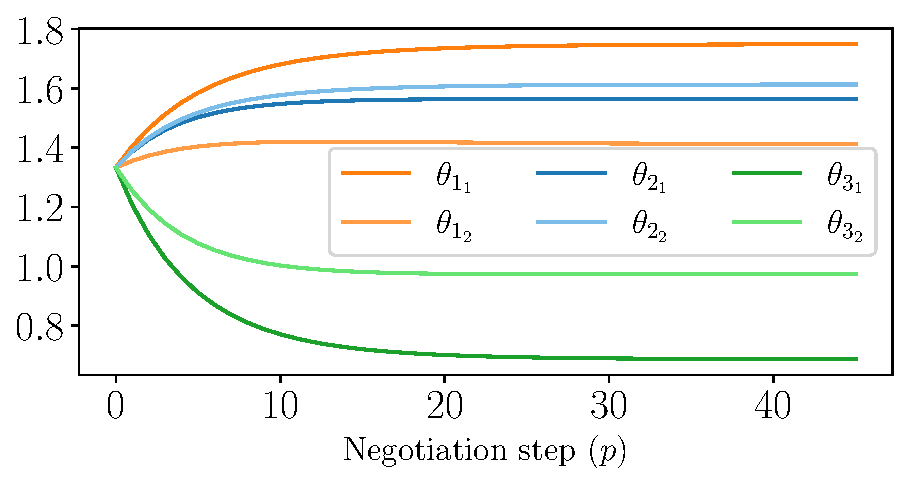
\includegraphics[width=\textwidth]{../img/example_primal_decomposition/example_theta.pdf}
    \caption{Evolution of $\thetai$ during iterative process.}\label{fig:example_theta}
  \end{subfigure}
  \hfill
  \begin{subfigure}{0.45\textwidth}
    \centering
    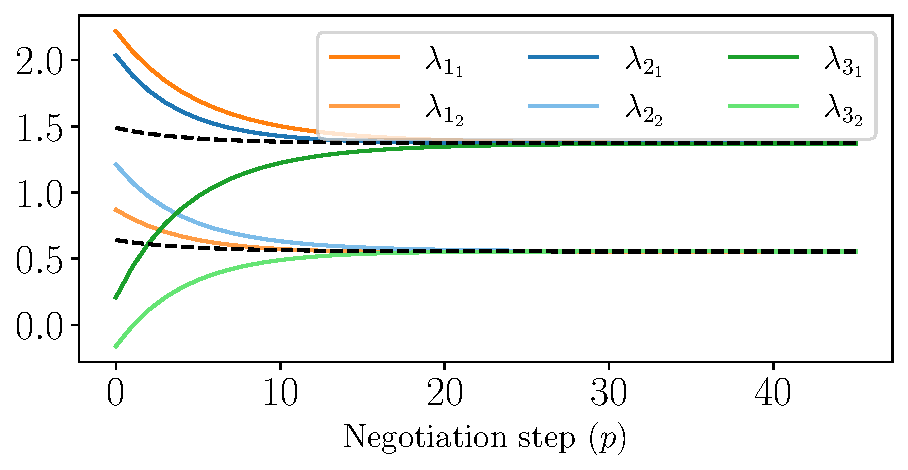
\includegraphics[width=\textwidth]{../img/example_primal_decomposition/example_lambda.pdf}
    \caption{Evolution of $\lambdai$ during iterative process.}\label{fig:example_lambda}
  \end{subfigure}
  \\~\\
  \begin{subfigure}{0.45\textwidth}
    \centering
    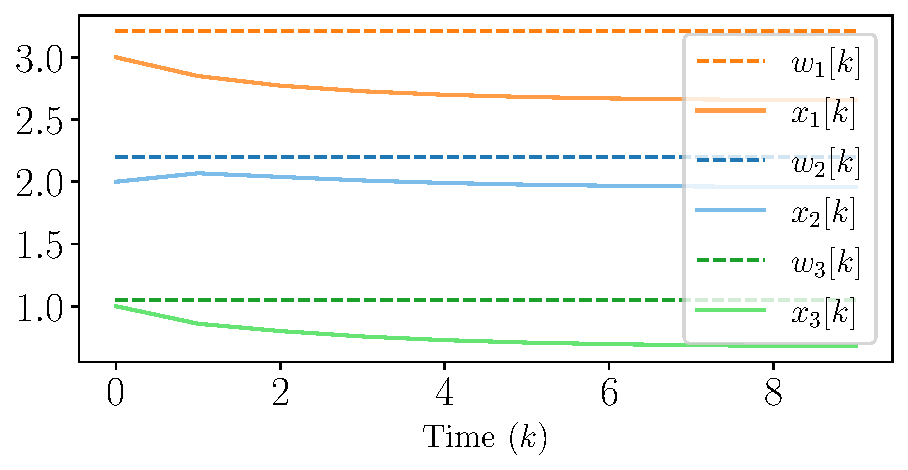
\includegraphics[width=\textwidth]{../img/example_primal_decomposition/example_state.pdf}
    \caption{Evolution of states $x_{i}[k]$ and references $w_{i}[k]$ during control ${k\in\set{K}}$.}\label{fig:example_state}
  \end{subfigure}
    \caption{Evolution of variables during iterative process and control.}\label{fig:example_variables}
\end{figure}
We can see in Fig.~\ref{fig:example_state} the evolution of states $x_{i}[k]$ during the simulation.
As we can perceive, the system cannot achieved the references due to the global coupling constraint, so all agents find a compromise and get as close to the reference as possible.

In Figs.~\ref{fig:example_theta} and~\ref{fig:example_lambda} the sub-systems were color-coded in nuances of orange for agent $1$, of blue for agent $2$, and of green for agent $3$.
Observe in Fig.~\ref{fig:example_theta} that the agent which has bigger values of $\lambdai$ has a corresponding $\thetai$ which increases with the iterations, and vice versa.

For $\lambdai$ we see it stabilizes when values for corresponding elements of the vector meet.
It is true due to the global equality constraint, whose simple projection onto the intersection of hyperplanes result in~\eqref{eq:example_projectedSubgradient_lambda}.
Moreover, as one can see, the iterative process converges if ${\thetai\pplusone=\thetai\p}$, which happens when ${\lambdai\p=\frac{1}{M}\sum_{j=1}^{M}\vec{\lambda}_j\p}$.
Although it may not necessarily be true for the inequality cases it gives us an insight of the functioning of the algorithm.
The values of $\thetai$ represent an allocation of the maximum input given to the agents by the coordinator, and $\lambdai$ is a measure of dissatisfaction of each agent to the value allocated.
So the coordinator has as role to negotiate the values of the allocations so all agents can be equally dissatisfied.
Due to this process of iterative allocations, other names given for this decomposition are \textbf{resource allocation} and \textbf{quantity decomposition}.

We can create a parallel with the cake-cutting problem~\cite{BramsTaylor1995} where two (or more) agents want to share a cake, dividing it equally so no agent envy the piece of cake of other agent.
Usually in these kinds of problems, a protocol is created where agents cut successively the cake (or parts of it) and the other agents take parts which they think it is the greater.
But in those cases usually all agents have the same hunger.

In our case, agents may have different needs, represented by the dynamics of the subsystems (tuples $(A_{i},B_{i})$), the matrices $\bar{\Gamma}_{i}$, state $x_{i}[k]$ and references $w_{i}[k]$.
So, the coordinator works as a mediator, positioning the cake cutter, showing where it would cut the cake (sending $\thetai$ during the iterative process), listening if the agents would be satisfied with the partition (receiveing $\lambdai$) and adjusting the cake cutter until a consensus is reached.
Due to this interpretation we call the iterative process as a \textbf{negotiation phase}.



\section[Anomalous behaviors and their consequences]{Anomalous behaviors and their consequences}\label{sec:vulnerabilities_PD}

Since the negotiation~\eqref{eq:projectedSubgradient_lambda} on the primal decomposition depends on $\thetaik$ and $\lambdaik$, the main source of vulnerabilities is the communication between local agents and coordinator.

For the equality case shown, it is clear to see that fluctuations in $\thetaik$ alter the results of local problems~\eqref{eq:example_local_problem}, and analogously, fluctuations in $\lambdaik$ alter the negotiation.
The same is true for the inequality case but not as straightforwad as inspecting equation~\eqref{eq:example_projectedSubgradient_lambda}.
An ill-intentioned local agent can exploit those facts to drive the negotiation by means of a \fdi{} attack.
However, the system could be implemented in such way that the final allocations agreed upon are distributed physically (valves and switches for instance).

With the physical distribution of allocation, \textbf{``Liar'' agent attacks} as in~\cite{VelardeEtAl2017b} are discouraged, since the attacker can not consume more than allocated (which would be beneficial for the attacker).
On the other hand, an attack in which an agent is forced to use less than the allocated would still be possible, but no agent would benefit, given that their allocation would not increase (allocations are fixed at the end of negotiation).
We will call this kind of attack where an agent is forced to deteriorate its own performance as a \textbf{Hijack agent} attack.
Moreover, during the following negotiations, the attacked agent would need more and more resources, increasing as consequence their dissatisfaction $\lambdaik$ forcing other agents to share more resources to the attacked agent.

We use the same example in~\S\ref{sec:example-interpr} but we modify agent $2$, so it does not use the resource allocated (agent does not apply $u_{2}^{\star}[0|k]$).
In Figs.~\ref{fig:example_liar_lambda1},~\ref{fig:example_liar_lambda5} and~\ref{fig:example_liar_lambda10} we can compare the values of $\vec{\lambda}_{2}$ for different time steps $k=0$, $k=4$ and $k=9$.
As we see, the values of $\vec{\lambda}_{2}$ increase as the time step $k$, driving as consequence all other values of $\lambdai$ and $\thetai$.
If we compare Fig.~\ref{fig:example_liar_state} with Fig.~\ref{fig:example_state} we see how the performance is degraded for all agents.
\begin{figure}[h]
  \centering
  \begin{subfigure}{0.45\textwidth}
    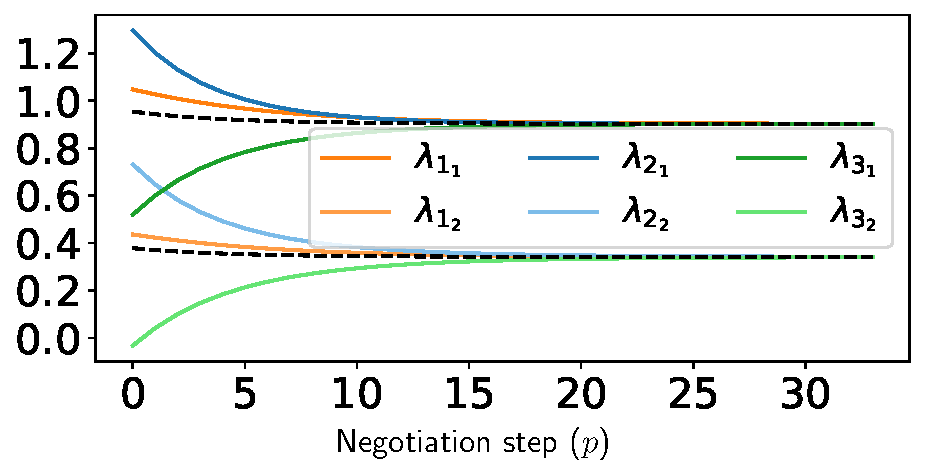
\includegraphics[width=\textwidth]{../img/example_primal_decomposition/example_liar_lambda_k_0.pdf}
    \caption{Case $k=0$.}\label{fig:example_liar_lambda1}
  \end{subfigure}
  \hfill
  \begin{subfigure}{0.45\textwidth}
    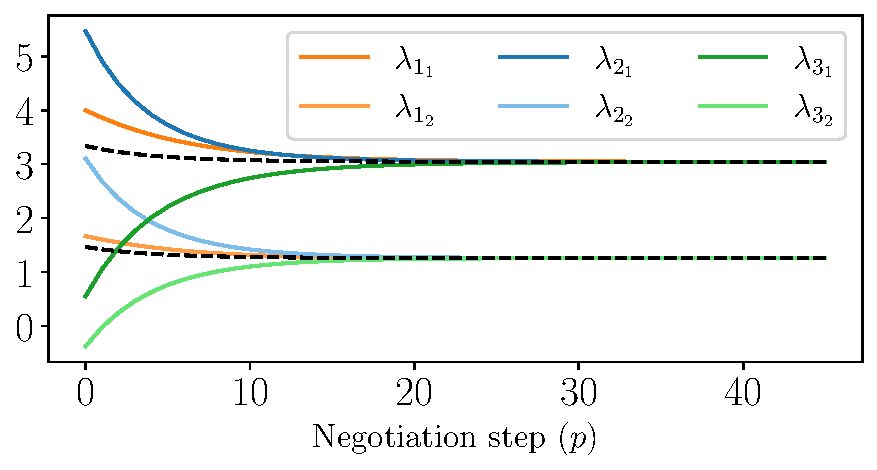
\includegraphics[width=\textwidth]{../img/example_primal_decomposition/example_liar_lambda_k_4.pdf}
    \caption{Case $k=4$.}\label{fig:example_liar_lambda5}
  \end{subfigure}
  \begin{subfigure}{0.45\textwidth}
    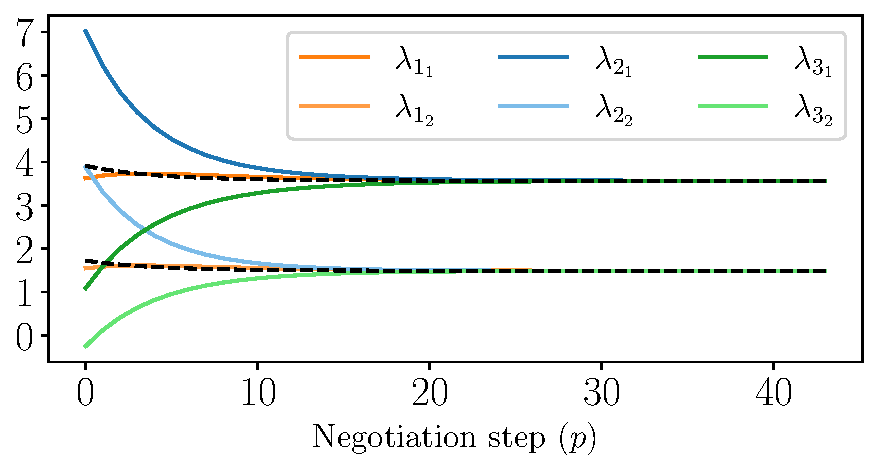
\includegraphics[width=\textwidth]{../img/example_primal_decomposition/example_liar_lambda_k_9.pdf}
    \caption{Case $k=9$.}\label{fig:example_liar_lambda10}
  \end{subfigure}
  \caption{Evolution of $\lambdai$ for different $k$ when agent $2$ is hijacked.}\label{fig:example_liar_lambdas}
\end{figure}

\begin{figure}[b]
  \centering
  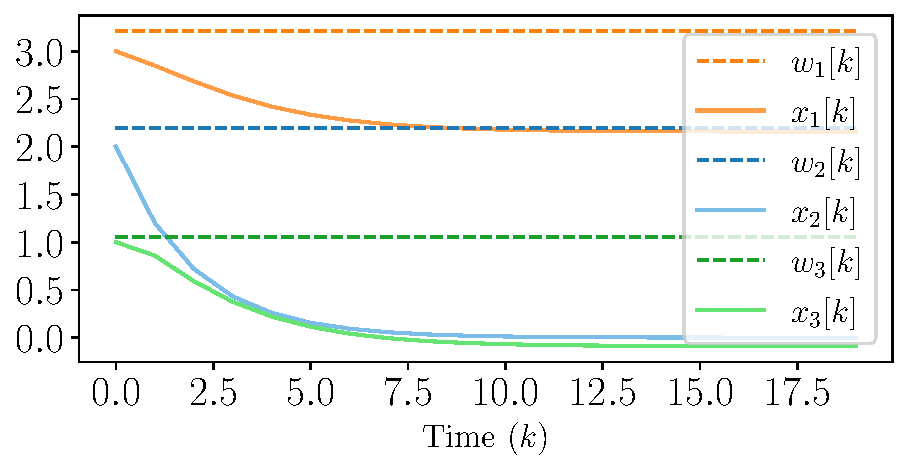
\includegraphics[width=.5\textwidth]{../img/example_primal_decomposition/example_liar_state.pdf}
  \caption{Evolution of state $x_{i}[k]$ and reference $w_{i}[k]$ during control when agent $2$ is hijacked.}\label{fig:example_liar_state}
\end{figure}


\subsection{Attack of interest}\label{sec:attack-interest}

As illustrated, the change in $\lambdai$ may cause a modification in the consensus and drive the negotiation.
Seeing that $\lambdai$ form a sub-gradient of the local problems~\eqref{eq:DOP_local}, it is perceivable that they carry information about the local problem, i.e.\ it has somehow embedded in itself information about the $5$-tuple $(H_{i},\vec{f}_{i}[k],\bar{\Gamma}_{i},\thetaik)$ which we will call the complete local information $\set{I}_{i}$.
So, every attack shown in~\cite{VelardeEtAl2018} (explained in \S\ref{sec:attacks_in_dmpc}) will somehow reflect into a modification in $\lambdai$.
And in the coordinator's perspective what matters is what it receives.

For this reason, we are interested in inter-agent \fdi{} attacks, in which one (or a group) of the agents changes its own $\lambdai$, so it can benefit at the expense of others.
We suppose that before a negotiation, the attacker chooses a function ${\gamma:\R^{c}\times\R\to \R^{c}}$, which can possibly vary with respect to time $k$, to modify $\lambdai$ before sending it to the coordinator.
This function aggregates any modification on the local information $\set{I}_{i}$.
Here we denote this modified version as
\begin{equation}
  \lambdaicheat=\gamma(\lambdaik,k).
\end{equation}

To facilitate future analysis, we suppose the attacker chooses a linear function such
\begin{equation}
  \label{eq:linear_attack}
  \lambdaicheat[k]=\gamma(\lambdaik,k)=\Tik\lambdaik.
\end{equation}

To ease communication, we will call the functions $\gamma_{i}$ and the matrices $\Tik$ as the \textbf{cheating} functions and matrices.

This attack can be seen as a general case of the selfish attack~\cite{VelardeEtAl2018},
where a positive constant multiplies the local objective function of the attacker.
This attack can be translated into a matrix
\begin{equation}
  \label{eq:selfish_attack}
  \Tik=\tau_{i}[k] I_{c}.
\end{equation}
As we will see, even being a simple attack, this attack can have some catastrophic consequences when associated with the negotiation dynamics.

To illustrate, we take again the same example system in~\S\ref{sec:example-interpr}.
We modify it so agent $3$ attacks using~\eqref{eq:selfish_attack}.
We simulate the system for different scenarios.
At each one of the scenarios agent $3$ uses a different cheating coefficient $\tau_{3}[k]$.

In Fig.~\ref{fig:example_vary_tau_objective} and~\ref{fig:example_vary_tau_objective_detail}, we accumulate the local objective functions
${\Jiacc=\sum\limits_{k\in\set{K}}\optobji(\optthetai[k])[k]}$
and also the total ${\Jacc=\sum\limits_{i\in\set{M}}J_{i}^{\text{acc}}}$ for different values of $\tau_{3}$.

\begin{remark}
  Here, as observed in Remark~\ref{rem:equivalence_problems_not_same_objective}, the objective functions $J_{i}^{\star}[k]$ and $J^{\star}[k]$ were calculated by reconstructing the original objective function~\eqref{eq:quadratic_objective_compact_batch}, i.e., calculating equivalent $c_{i}[k]$ for each subsystem and using
  \begin{equation}
    \optobji[k] = 2\eqoptobji[k] + c_{i}[k].
\end{equation}
\end{remark}

Observe (Fig.~\ref{fig:example_vary_tau_objective_detail}) that $\Jacc$ has its least value when $\tau_{3}=1$, i.e., when there is no attack.
When $\tau_{3}$ increases, the objective function of the attacker ($\Jiacc[3]$) decreases while all other increase.
We see the opposite happening for values of $\tau_{3}$ between $0$ and $1$.
In this case the attacker deteriorates its own performance, what would not justify such attack, unless in a hijack scenario.

\begin{figure}[h]
  \centering
  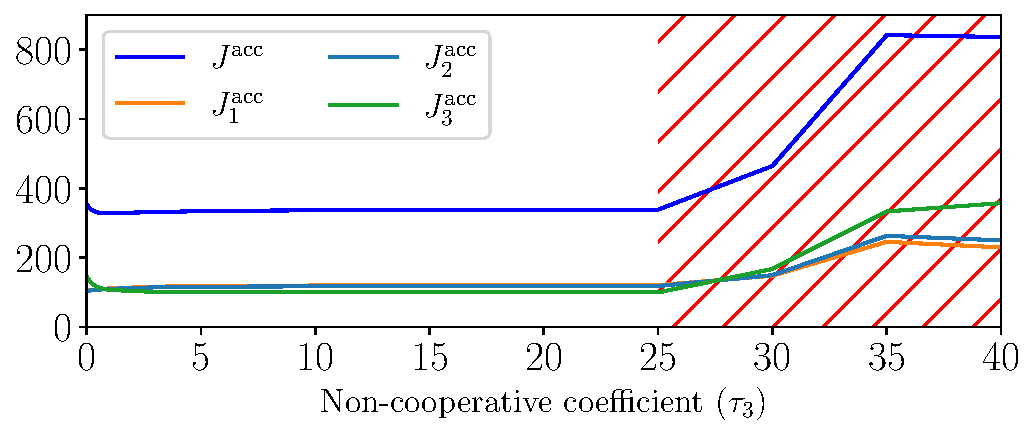
\includegraphics[width=.5\textwidth]{../img/example_primal_decomposition/example_vary_tau_J.pdf}
  \caption{Accumulate objective functions for different values of $\tau_{3}$. \todo{remake figure}}\label{fig:example_vary_tau_objective}
\end{figure}

\begin{figure}[h]
  \centering
  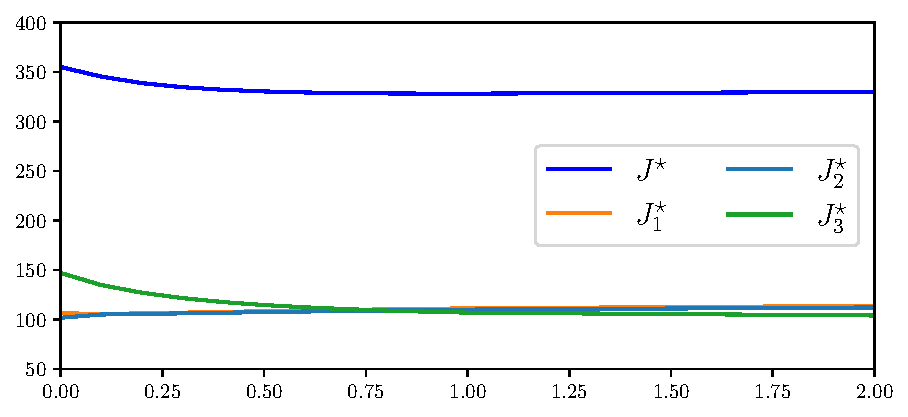
\includegraphics[width=.5\textwidth]{../img/example_primal_decomposition/example_vary_tau_J_detail.pdf}
  \caption{Accumulate objective functions for different values of $\tau_{3}$ (detail). \todo{remake figure}}\label{fig:example_vary_tau_objective_detail}
\end{figure}

Other fact we can see in Fig.~\ref{fig:example_vary_tau_objective} is in its right side (hatched in red). The objectives seem to find an equilibrium but after a given value of $\tau_{3}$ it increases more and more.
This is caused by a collapse in the negotiation.
The agents cannot find a consensus anymore.
To illustrate, we present the negotiation of $\lambdai$ for $3$ different values of $\tau_{3}$ (Figs.~\ref{fig:example_vary_tau_lambda_tau_1} to~\ref{fig:example_vary_tau_lambda_tau_20}).

% TODO(accacio):maybe put in a same figure.
\begin{figure}[h]
  \centering
  \begin{subfigure}{0.45\textwidth}
    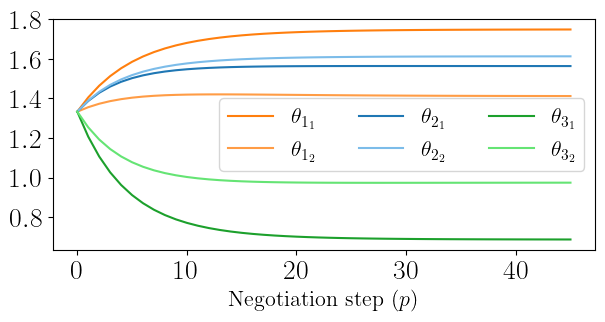
\includegraphics[width=\textwidth]{../img/example_primal_decomposition/example_theta.png}
    \caption{$\tau_{3}=1$. \todo{remake figure}}\label{fig:example_vary_tau_lambda_tau_1}
  \end{subfigure}
  \begin{subfigure}{0.45\textwidth}
    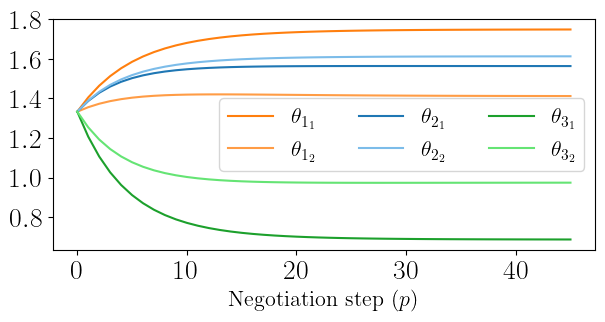
\includegraphics[width=\textwidth]{../img/example_primal_decomposition/example_theta.png}
    \caption{$\tau_{3}=5$. \todo{remake figure}}\label{fig:example_vary_tau_lambda_tau_5}
  \end{subfigure}
  \\~\\
  \begin{subfigure}{0.45\textwidth}
    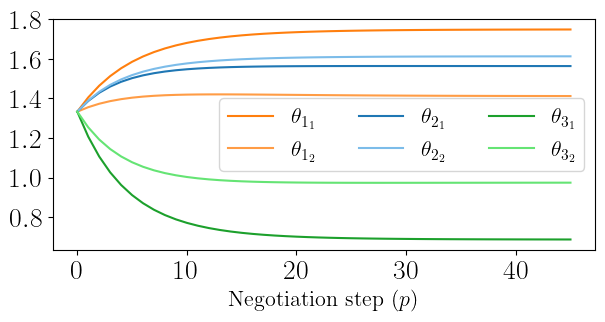
\includegraphics[width=\textwidth]{../img/example_primal_decomposition/example_theta.png}
    \caption{$\tau_{3}=20$. \todo{remake figure}}\label{fig:example_vary_tau_lambda_tau_20}
  \end{subfigure}
    \caption{Evolution of $\lambdai$ during negotiation for $k=5$ with different values of $\tau_{3}$.}\label{fig:example_vary_tau_lambda}
\end{figure}
As we can see, as $\tau_{3}$ increases, the negotiation presents a dampened oscillatory behavior.
The dampening decreases if $\tau_{3}$ continues to rise, until the negotiation oscillates and no consensus is reached, breaking down the \dmpc{} and maybe causing damage to the plant.

\section{Conclusion}\label{sec:conclusion}
In this chapter, we presented the primal decomposition-based \dmpc{}, and its vulnerabilities.
We also provided means by which an ill-intentioned agent could exploit said vulnerabilities and their main effects.
As we have seen the main consequences are loss in global performance and complete mal-function of the system.

Degradation of global performance, when working with \cps{}, in the best of the scenarios can cause little to no discomfort for a group of users, but an eventual breakdown, may endanger the users.
So, we desire to avoid both phenomena whenever possible.
In the next chapters we will analyze the problem and discuss what we can do to avoid such effects.

\end{document}
